\documentclass[12pt,fleqn]{article}\usepackage{../common}
\begin{document}
Kovaryans ve Korelasyon

Harvard Joe Blitzstein dersinden alinmistir

Bugun ``kovaryans gunu'', bu teknigi kullanarak nihayet bir toplamin
varyansini bulabilecegiz, varyans lineer degildir (kiyasla beklenti
-expectation- lineerdir). Bu lineer olmama durumu bizi korkutmayacak tabii,
sadece yanlis bir sekilde lineerlik uygulamak yerine probleme farkli bir
sekilde yaklasmayi ogrenecegiz. 

Diger bir acidan, hatta bu ana kullanimlardan biri, kovaryans iki rasgele
degiskeni beraber / ayni anda analiz etmemize yarayacak. Iki varyans
olacak, ve onlarin alakasina bakiyor olacagiz, bu sebeple bu analize {\em
  ko}varyans deniyor zaten. 

Tanim

$$ Cov(X,Y) = E((X-E(X))(Y-E(Y))) \mlabel{1} $$

Burada $X,Y$ ayni uzayda tanimlanmis herhangi iki rasgele degisken. Ustteki
diyor ki rasgele degisken $X,Y$'in kovaryansi $X$'ten ortalamasi
cikartilmis, $Y$'ten ortalamasi cikartilmis halinin carpilmasi ve tum bu
carpimlarin ortalamasinin alinmasidir.

Tanim boyle. Simdi bu tanima biraz bakip onun hakkinda sezgi / anlayis
gelistirmeye ugrasalim. Tanim niye bu sekilde yapilmis, baska bir sekilde
degil?

Ilk once esitligin sag tarafindaki bir carpimdir, yani ``bir sey carpi bir
baska sey''. Bu ``seylerden'' biri $X$ ile digeri $Y$ ile alakali, onlari
carparak ve carpimin bir ozelliginden faydalanarak sunu elde ettik; arti
carpi arti yine arti degerdir, eksi carpi arti eksidir, eksi carpi eksi
artidir. Bu sekilde mesela ``ayni anda arti'' olmak gibi kuvvetli bir
baglanti carpimin arti olmasi ile yakalanabilecektir. Ayni durum eksi,eksi
de icin gecerli, bu sefer her iki rasgele degisken ayni sekilde
negatiftir. Eksi carpim sonucu ise sifirdan az bir degerdir, ``kotu
korelasyon'' olarak alinabilir ve hakikaten de eksi arti carpiminin isareti
oldugu icin iki degiskenin ters yonlerde oldugunu gosterir. Demek ki bu
arac / numara hakikaten faydali.

Unutmayalim, ustteki carpimlardan birisinin buyuklugu $X$'in ortalamasina
bagli olan bir diger, $Y$ ayni sekilde. Simdi $X,Y$'den bir orneklem
(sample) aldigimizi dusunelim. Veri setinin her veri noktasi bagimsiz ve
ayni sekilde dagilmis (i.i.d) durumda. Yani $X,Y$ degiskenlerine ``gelen''
$x_i,y_i$ ikilileri her $i$ icin digerlerinden bagimsiz; fakat her ikilinin
arasinda bir baglanti var, yani demek ki bu rasgele degiskenlerin baz
aldigi dagilimlarin bir alakasi var, ya da bu iki degiskenin bir birlesik
dagilimi (joint distribution) var.

Not: Eger $X,Y$ bagimsiz olsaydi, o zaman 

$$ Cov(X,Y) = E((X-E(X))E(Y-E(Y))  $$

olarak yazilabilirdi, yani iki beklentinin ayri ayri carpilabildigi
durum... Ama biz bu derste bagimsizligin olmadigi durumla ilgileniyoruz..

Korelasyon kelimesinden bahsedelim hemen, bu kelime gunluk konusmada cok
kullaniliyor, ama bu ders baglaminda korelasyon kelimesinin matematiksel
bir anlami olacak, onu birazdan, kovaryans uzerinden tanimlayacagiz.

Bazi ilginc noktalar:

Ozellik 1

varyansi nasil tanimlamistik? 

$$ Var(X) = E((X-E(X))^2)  $$

Bu denklem aslinda 

$$ Cov(X,Y) = E((X-E(X))(Y-E(Y)))  $$

denkleminde $Y$ yerine $X$ kullandigimizda elde ettigimiz seydir, yani

$$ Cov(X,X) = E((X-E(X))(X-E(X)))  $$

$$ Cov(X,X) = E((X-E(X))^2)   $$

$$ = Var(X) $$

Yani varyans, bir degiskenin ``kendisi ile kovaryansidir''. Ilginc degil
mi? 

Ozellik 2

$$ Cov(X,Y) = Cov(Y,X) $$

Ispati kolay herhalde, (1) formulunu uygulamak yeterli.

Teori

$$ Cov(X,Y) = E((X-E(X))(Y-E(Y))) = E(XY) - E(X)E(Y)$$

Ispat

Bu ispat cok kolay, esitligin sol tarafindaki carpimi parantezler uzerinden
acarsak, ve beklenti lineer bir operator oldugu icin toplamin terimleri
uzerinde ayri ayri uygulanabilir, 

$$ E(XY) -E(X)E(Y) -E(X)E(Y) + E(X)E(Y) $$

$$  =  E(XY) - E(X)E(Y) $$

Carpimi uygularken mesela $E(-X \cdot E(Y))$ gibi bir durum ortaya cikti,
burada $E(Y)$'nin bir sabit oldugunu unutmayalim, cunku beklenti rasgele
degiskene uygulaninca tek bir sayi ortaya cikartir, ve vu $E(Y)$ uzerinde
bir beklenti daha uygulaninca bu ``icerideki'' beklenti sabitmis gibi
disari cikartilabilir, yani $-E(X)E(Y)$. 

Devam edelim, $E(XY) - E(X)E(Y)$ ifadesini gosterdik, cunku cogu zaman bu
ifade hesap acisindan (1)'den daha uygundur. Ama (1) ifadesi anlatim /
sezgisel kavrayis acisindan daha uygun, cunku bu ifade $X$'in ve $Y$'nin
kendi ortalamalarina izafi olarak belirtilmistir, ve akilda canlandirilmasi
daha rahat olabilir. Fakat matematiksel olarak bu iki ifade de aynidir. 

Iki ozellik bulduk bile. Bir ozellik daha,

Ozellik 3

$$ Cov(X,c) = 0 $$

Bu nereden geldi? (1)'e bakalim, $Y$ yerine $c$ koymus olduk, yani bir
sabit. Bu durumda (1)'in $(Y-E(Y))$ kismi $c-E(c)=c-c=0$ olur [aslinda
bayagi absurt bir durum], ve bu durumda (1) tamamen sifira donusur, sonuc sifir.

Ozellik 4

$Cov(cX,Y) = c \cdot Cov(X,Y)$ 

Ispat icin alttaki formulde

$$ Cov(X,Y) =  E(XY) - E(X)E(Y) $$

$X$ yerine $cX$ koymak yeterli, $c$ her iki terimde de disari cikacaktir,
ve grubun disina alincan bu ozelligi elde ederiz.

Ozellik 5

$$ Cov(X,Y+Z) = Cov(X,Y) + Cov(X,Z) $$

Ispat icin bir ustteki ozellikte yaptigimizin benzerini yapariz. 

En son iki ozellik oldukca faydalidir bu arada, onlara ikili-lineerlik
(bilinearity) ismi veriliyor. Isim biraz renkli / sukseli bir isim,
soylemek istedigi su aslinda, bu son iki ozellikte sanki bir kordinati
sabit tutup digeri ile islem yapmis gibi oluyoruz, yani bir kordinat sabit
olunca digeri ``lineermis gibi'' oluyor; Mesela $c$'nin disari ciktigi
durumda oldugu gibi, bu ozellikte $Y$'ye hicbir sey olmadi, o degismeden
kaldi. Ayni sekilde 5. ozellikte $X$ hic degismeden esitligin sagina
aktarildi sanki, sadece ``$Z$ durumu icin'' yeni bir terim ekledik. 

4. ve 5. ozellik cok onemlidir, bunlari bilirseniz bir ton hesabi yapmadan
hizlica tureterek hesaplarinizi kolaylastirabilirsiniz. 

Ozellik 6

$$ Cov(X+Y, Z+W) = Cov(X,Z) + Cov(X,W) + Cov(Y,Z) + Cov(Y,W) $$

Simdi 5. ozelligi hatirlayalim, orada gosterilen sanki bir nevi basit
cebirdeki dagitimsal (distributive) kuralin uygulanmasi gibiydi sanki, yani
$(a+b)(c+d)$'i actigimiz gibi, 5. ozellik te sanki kovaryansi carpip
topluyormus gibi ``aciyordu''. En temelde gercekten olan bu degil ama nihai
sonuc benzer gozuktugu icin akilda tutmasi kolay bir metot elde etmis
oluyoruz. Her neyse, 6. ozellik icin aslinda 5. ozelligi tekrar tekrar
uygulamak yeterli. Bu arada 5. ozellik $Cov(X,Y+Z)$ icin ama $Cov(Y+Z,X)$
yine ayni sonucu veriyor. 

Bu arada 6. ozellik cok cetrefil toplamlar uzerinde de uygulanabilir,
mesela 

$$ Cov \bigg( \sum _{i=1}^{m}a_iX_i, \sum _{j=1}^{n}b_iY_i \bigg) $$

Bu son derece karmasik gozukuyor, fakat cozumu icin aynen 6. ozellikte
oldugu gibi 5. ozelligi yine tekrar tekrar uygulamak yeterli (4. ozellik
ile de sabiti disari cikaririz, vs).

Cogu zaman ustteki gibi pur kovaryans iceren bir acilimla calismak, icinde
beklentiler olan formullerle ugrasmaktan daha kolaydir. 

Simdi toplamlara donelim; kovaryanslara girmemizin bir sebebi toplamlarla
is yapabilmemizi saglamasi. Mesela, bir toplamin varyansini nasil
hesaplariz? 

Ozellik 7

$$ Var(X_1+X_2) $$

Simdilik iki degisken, ama onu genellestirip daha fazla degiskeni
kullanabiliriz. 

Cozelim. 1. ozellik der ki varyans degiskenin kendisi ile kovaryansidir,
yani $Var(X) = Cov(X,X)$. O zaman $Var(X_1+X_2) = Cov(X_1+X_2,
X_1+X_2)$. 
Boylece icinde toplamlar iceren bir kovaryans elde ettik ama bunu cozmeyi 
biliyoruz artik. ``Dagitimsal'' islemleri yaparken $Cov(X_1,X_1)$ gibi
ifadeler cikacak, bunlar hemen varyansa donusecek. Diger taraftan
$Cov(X_1,X_2)$ iki kere gelecek, yani

$$ Var(X_1+X_2) = Var(X_1) + Var(X_2)  + 2 Cov(X_1,X_2)$$

Bu alanda bilinen tekerleme gibi bir baska deyis, ``eger kovaryans sifirsa
toplamin varyansi varyanslarin toplamidir''. Hakikaten kovaryans sifir
olunca ustteki denklemden dusecektir, geriye sadece varyanslarin toplami
kalacaktir. Kovaryans ne zaman sifirdir? Eger $X_1,X_2$ birbirinden
bagimsiz ise. Tabii bu bagimsizlik her zaman ortaya cikmaz. 

Ikiden fazla degisken olunca? Yine tum varyanslarin ayri ayri toplami, ve
kovaryanslar da sonda toplanacak,

$$ Var(X_1+ .. + X_n ) = Var(X_1) + .. + Var(X_n) + 2 \sum _{i<j}^{} Cov(X_i,X_j) $$
Sondaki toplamin indisinde bir numara yaptik, sadece 1 ile 2, 2 ile 3,
vs. eslemek icin, ve mesela 3 ile 1'i tekrar eslememek icin. Tekrar dedik
cunku $Cov(X_1,X_3) = Cov(X_3,X_1)$. Eger indisleme numarasi
kullanmasaydik, 2 ile carpimi cikartirdik (ona artik gerek olmazdi),

$$ ..  + \sum _{i \ne j} Cov(X_i,X_j) $$

Simdi, korelasyon konusuna gelmeden once, bagimsizlik kavramini iyice
anladigimizdan emin olalim. a 

Teori

Eger $X,Y$ bagimsiz ise bu degiskenler bagimsizdir, yani $Cov(X,Y)=0$.

DIKKAT! Bu mantik cizgisinin tersi her zaman dogru olmayabilir, yani
bagimsizlik kesinlikle $Cov(X,Y)=0$ demektir, ama her $Cov(X,Y)=0$ oldugu
zaman ortada bir bagimsizlik var diyemeyiz. Bunu bir ornekle gorelim. 

$$ Z \sim N(0,1), X=Z, Y=Z^2 $$

Simdi $X,Y$ kovaryansinin hesabi yapalim

$$ Cov(X,Y) = E(XY) - E(X)E(Y) = E(Z^3) - E(Z)E(Z^2)$$

En sondaki terim sifirdir, cunku hem $E(Z)$ ve $E(Z^3)$ sifirdir [hoca
burada standart normalin tek sayili (odd) moment'leri hep sifirdir dedi]. O
zaman su sonucu cikartiyoruz, $X,Y$ arasinda korelasyon yok. 

Ama bagimlilik var mi? Var. Cunku hem $X$ hem $Y$ $Z$'nin birer degiskeni,
yani bu durumda $X$'i bilmek bize $Y$'yi tamamen bilmemizi sagliyor (sadece
ek olarak bir kare aliyoruz). Tabii bagimlilik illa herseyin bilinmesi
demek degildir, biraz bagimlilik ta olabilir, ama biraz bagimlilik bile
varsa, bagimsizlik var diyemeyiz. Ayni sey ters yon icin de gecerli, $Y$
bilinince $X$'in ``buyuklugunu'' bilebiliriz, karekok islemi oldugu icin
-/+ isareti bilemeyiz ama skalar bir buyuklugu elde edebiliriz. Yani ters
yonde de bagimsizlik yoktur. 

Korelasyon

Tanim

$$ Corr(X,Y) = \frac{Cov(X,Y)}{SD(X)SD(Y)} 
\mlabel{2}
$$

Bu arada hatirlarsak ustte SD ile gosterilen standart sapma, varyansin
karesidir. 

Bu tanim genelde kullanilan tanimdir. Fakat ben daha farkli bir tanimi
tercih ediyorum. Standardize etmeyi hatirliyoruz degil mi? Bir rasgele
degiskenden ortalamasini cikartip standart sapmaya bolunce standardize
ediyorduk. Bunu kullanarak aslinda korelasyonu alttaki gibi
tanimlayabiliriz, 

$$ Corr(X,Y) = Cov \bigg( \frac{X-E(X)}{SD(X)}, \frac{Y-E(Y)}{SD(Y)}
\bigg) 
\mlabel{3}
$$

Yani korelasyonun anlami aslinda sudur: $X,Y$ degiskenlerini standardize
et, ondan sonra kovaryanslarini al. 

Niye kovaryans iceren ifadeyi tercih ediyoruz? Cunku, diyelim ki $X,Y$
degiskenleri bir uzaklik olcusunu temsil ediyor, ve birimleri mesela
nanometre. Fakat bir baskasi gelip ayni olcumu, atiyorum, isik yili olarak
kullanmaya baslarsa problem cikabilir. Yani eger birim yoksa ve ben ``$X,Y$
korelasyonum 42'' dersem, bunun ne oldugunu anlamak zordur. 42 onumuzdeki
veriye gore kucuk mudur, buyuk mudur? Bilemeyiz. Yani 42 sayisi tabii ki
evrendeki tum sorularin cevabidir [hoca bir filme atfen espri yapiyor,
orada 42 sayisinin ozel bir anlami vardi], ama onumuzdeki problem icin,
nedir? 

Fakat ustteki formul olcu birimsiz (dimensionless) bir sonuc verir, yani
bir olcu biriminden bahsetmeden birine rahatca aktarabilecegimiz bir
bilgidir. Niye birimsiz oldu? Cunku $X$'in birimi $cm$ olsa, $X-E(X)$ yine
$cm$, $SD(X)$ varyansin karekoku oldugu icin $cm^2$'nin karekoku yine $cm$,
$cm$ bolu $cm$ birim ortadan kalkar.

Bu arada (3) niye (2) ile aynidir? Eger bir rasgele degiskenden bir sabiti
cikartirsam onun baska bir degisken ile kovaryansini degistirmis olmam. Ki
standardize etme islemi bunu yapar. O zaman niye bu cikartma islemini
yaptim? Cunku standardize etme islemini ozellikle kullanmak istedim -
standardizasyon bilinen ve rahatca kullanilabilen bir islem. Standart
sapmayi bolmeye gelirsek, simdiye kadar gordugumuz ozelliklerden biri,
bolumu disari alabilecegimizi gosteriyor, boyle olunca (2) ifadesini aynen
elde ediyorum. 

[Not: cok ilginc bir noktaya isaret etmek isterim. Hoca $X,Y$'yi
standardize etti, ama bu demek degil ki $X,Y$ ``standard normal'' dagilimi
haline geldi, $X,Y$'in eger kendileri normal olsaydi o zaman standart
normal elde ederdik. Diger durumlarda $X,Y$'yi ortalamasi 0, varyansi 1
olan bir sey haline getirmis olduk sadece. Ama yine bu dusunceden devam
edersek, eger $X,Y$ normal olsaydi, standardize bize iki tane $Z$ verirdi,
ve $Cov(Z,Z)=1$ olurdu. Yani hangi sekilde olursa olsun eger $X,Y$'nin
ikisi de normal ise korelasyon 1 demektir].

Onemli bir nokta daha: korelasyon her zaman $-1$ ve $+1$ arasindadir. 

Teori

$$ -1 \le Corr(X,Y) \le 1 $$

Yani olcu biriminden bagimsiz olmasi avantajina ek olarak hep ayni skalada
olan bir degerin rapor edilmesi de faydalidir. Eger korelasyon 0.99
bulursam bunun hemen yuksek bir korelasyon oldugunu bilirim. 

Bu arada, Cauchy-Schwarz esitsizliginden bahsedeyim -ki bu esitsizlik
tanimi tum matematikteki en onemli esitsizliklerden biridir- eger
korelasyon formulunu lineer cebirsel sekilde ifade etseydim direk
Cauchy-Schwarz esitsizligini elde ederdim. 

Ispat

Once ``WLOG cercevesinde'' $X,Y$'nin onceden standardize edilmis oldugunu
kabul edelim. [WLOG ne demek? Matematikciler ispatlar sirasinda bunu bazen
kullanirlar, genelleme kuvvetinde bir kayip olmadan (without loss of
generality) takip eden seyi kullanabiliriz demektir, yani ``bir baska sey
kullaniyorum, ama teori bu cercevede de hala gecerli'' demek isterler]. 

Onceden standardize edildigini kabul etmek niye fark yaratmiyor? Cunku bunu
gorduk, standart olmayan degiskenleri standardize edince yine ayni sonucu
elde ediyorum, yani bir sey farketmiyor. 

$Var(X+Y)$'i hesaplayalim. 

$$ Var(X+Y) = Var(X) + Var(Y) + 2Cov(X,Y) 
\mlabel{4}
$$

Simdi sembol olarak $\rho = Corr(X,Y)$ kullanalim,

Standardize ettigimizi kabul etmistik, o zaman $Var(X)=1,Var(Y)=1$. Ayrica
(3)'te gordugumuz uzere, standardize durumda kovaryans korelasyona esittir,
o zaman $Cov(X,Y)=\rho, yani 2Cov(X,Y) = 2\rho$. Tum ifade,

$$ Var(X+Y) = 1 + 1 + 2 \rho  = 2 + 2\rho$$

Peki farklarin varyansi, $Var(X-Y)$ nedir? Bir numara kullanalim,
$Var(X-Y)$'i $Var(X+(-Y))$ olarak gorelim, 

$$ Var(X-Y) = Var(X) + Var(Y) - 2Cov(X,Y) = 2 - 2\rho $$

Aslinda bu son ifade ispati tamamlamis oldu, cunku varyans negatif olmayam
bir seydir, yani 

$$ 0 \le Var(X+Y) = 2 + 2\rho$$

$$ 0 \le Var(X-Y) = 2 - 2\rho$$

Bu iki esitsizligi kullanarak 

$$ -2 \le 2\rho$$

$$ -2 \le - 2\rho$$

ve 

$$ -1 \le \rho$$

$$ \rho \le 1 $$


Multinom Dagilimin Kovaryansi

Kovaryansi multinom dagilimi baglaminda ele alalim, bildigimiz gibi
multinom dagilimi bir vektordur [ve binom dagiliminin daha yuksek boyuttaki
halidir, binom dagilimi bildigimiz gibi $n$ deney icinde kac tane basari
sayisi oldugunu verir], ve vektorun her hucresinde ``vs. kategorisinde kac
tane vs var'' gibi bir deger tasinir, ki bu her hucre baglaminda ``o
kategori icin zar atilsa kac tane basari elde edilir'' gibi okunabilir. 

Biz ise bu hucrelerden iki tanesini alip aralarindaki kovaryasyona bakmak
istiyoruz. Gayet dogal bir istek. 

Notasyon

Elimizde $k$ tane obje var, 

$$ (X_1,..,X_k) \sim Mult(n,\vec{p}) $$

Dikkat, $p$ bir vektor, tabii ki, cunku binom durumunda $p$ tek sayi idi,
simdi ``pek cok $p$''ye ihtiyac var. 

Her $i,j$ icin $Cov(X_i,X_j)$'yi hesapla. 

Eger $i=j$ ise $Cov(X_i,X_i)=Var(X_i) = np_i(1-p_i)$. 

ki son ifade binom dagiliminin varyansidir. Bu basit durum tabii ki, ilginc
olan $i \ne j$ olmadigi zaman. 

Tek ornek secelim, mesela $Cov(X_1,X_2)$, buradan gelen sonuc gayet kolayca
genellestirilebilir. 

Hesaba baslamadan once kabaca bir akil yurutelim; $Cov(X_1,X_2)$ icin arti
mi eksi mi bir deger elde ederdik acaba? Multinom dagilimi hatirlayalim,
belli sayida ``sey'' yine belli sayida kategori arasinda ``kapisiliyor'',
yani bu kategoriler arasinda bir yaris var. O zaman herhangi iki
kategorinin kovaryansinin negatif olmasini bekleriz. 

Cozum icin (4) formulunu kullanacagim, ama secici bir sekilde, 

$$ Var(X+Y) = Var(X) + Var(Y) + 2Cov(X,Y) $$

icinde $Var(X+Y),Var(X),Var(Y)$'i biliyorsam, geriye bilinmeyen $Cov(X,Y)$
kalir. Kisaltma amaciyla $c = Cov(X,Y)$ diyelim,

$$ Var(X_1+X_2) = np_1(1-p_1) + np_2(1-p_2) + 2c$$

Simdi $X_1+X_2$'nin ne oldugunu dusunelim, bu yeni rasgele degisken ``ya
kategori 1 ya da 2'' sonucunu tasiyan bir degiskendir, ki bu da yeni bir
``birlesik'' binom degiskenidir. Bu degiskenin $p$'si toplami oldugu iki
kategorinin $p$'sinin toplamidir, yani $p_1+p_2$. O zaman bu yeni
degiskenin varyansi, 

$$ Var(X_1+X_2) = n(p_1+p_2)(1-(p_1+p_2))  $$

Eh artik denklemdeki her seyi biliyoruz, sadece $c$'yi bilmiyoruz, ona gore
herseyi duzenleyelim, 

$$ n(p_1+p_2)(1-(p_1+p_2))  = np_1(1-p_1) + np_2(1-p_2) + 2c $$

Burada biraz haldir huldur islem lazim [bu kismi okuyucu isterse
yapabilir], sonuc

$$ Cov(X_1,X_2) = -np_1p_2 $$

Genel olarak 

$$ Cov(X_i,X_j) = -np_ip_j, \forall i \ne j $$

Dikkat edin, bu sonuc her zaman negatiftir (cunku $p$ degerleri olasilik
degerleridirler, yani pozitif olmak zorundadirlar)

Ornek

Binom degiskenin varyansini hesaplayalim simdi. Bunu daha once yapmistik
ama gostergec (indicator) rasgele degiskenleri kullanarak yapmistik bunu,
simdi elimizde yeni bir arac var, onu kullanalim. Varacagimiz sonuc 
$Var(X) = npq$ olacak. Tanimlar,

$$ X \sim Bin(n,p), X = X_1+..+X_n $$

ki $X_i$ degiskenleri i.i.d. Bernoulli. 

Aslinda her $X_i$ degiskeni bir gostergec degiskeni gibi
gorulebilir. Diyelim ki bir $A$ olayi icin gostergec degisken $I_A$
olsun. Bu durumda

$$ I_A^2 = I_A $$

$$ I_A^3 = I_A $$

Degil mi? Gostergec sadece 1/0 olabiliyorsa onun karesi, kupu ayni sekilde
olur. Bunu vurguluyorum, cunku bazen atlaniyor. 

Peki $I_AI_B$? Ki $A,B$ ayri ayri olaylar. Gayet basit, 

$$ I_AI_B = I_{A \cap B} $$

Bu normal degil mi? Esitligin solundaki carpim sadece her iki degisken de 1
ise 1 sonucunu verir, bu ise sadece $A,B$ olaylari ayni anda oldugu zaman
mumkundur, ki bu ayni anda olmak kume kesismesinin tanimidir. 

Bernoullli durumuna donelim, her Bernoulli icin

$$ Var(X_i) = EX_j^2 - E(X_j)^2 $$

$X_j^2 = X_j$'dir, bunu biraz once gorduk, ve Binom degiskenleri gostergec
gibi goruyoruz, o zaman $EX_j^2 = E(X_j) = p$. 

$$ Var(X_i) = p - p^2 = p(1-p) = pq$$

Tum binom dagilimin varyansi, 

$$ Var(X) = npq $$

Bu kadar basit. Cunku $Cov(X_i,X_j)=0,\forall i \ne j$, yani her bernoulli
deneyi birbirinden bagimsiz, o sebeple binom varyansi icin tum bernoulli
varyanslarini toplamak yeterli, eger varyansi $pq$ olan $n$ tane bernoulli
varsa, binom varyansi $npq$. 

Ornek

Daha zor bir ornegi gorelim. 

$$ X \sim HGeom(w,b,n) $$

Bu bir hipergeometrik dagilim. Parametreleri soyle yorumlayabiliriz, bir
kutu icinde $w$ tane beyaz top var, $b$ tane siyah top var, ve biz bu
kutudan $n$ buyuklugunde bir orneklem aliyoruz, ve ilgilendigimiz
orneklemdeki beyaz toplarin dagilimi. 

[dersin gerisi atlandi]

Verisel Kovaryans (Empirical Covariance) 

Eger verinin kolonlari arasindaki iliskiyi gormek istersek, en hizli yontem
matristeki her kolonun (degiskenin) ortalamasini kendisinden cikartmak,
yani onu ``sifirda ortalamak'' ve bu matrisin devrigini alarak kendisi ile
carpmaktir. Bu islem her kolonu kendisi ve diger kolonlar ile noktasal
carpimdan gecirecektir ve carpim, toplama sonucunu nihai matrise
yazacaktir. Carpimlarin bildigimiz ozelligine gore, arti deger arti degerle
carpilinca arti, eksi ile eksi arti, eksi ile arti eksi verir, ve bu bilgi
bize ilinti bulma hakkinda guzel bir ipucu sunar. Pozitif sonucun pozitif
korelasyon, negatif ise tersi sekilde ilinti oldugu sonucuna boylece
kolayca erisebiliriz.

Tanim

$$ S = \frac{1}{n} (X-E(X))^T(X-E(X))) $$

Pandas ile \verb!cov! cagrisi bu hesabi hizli bir sekilde yapar,

\begin{minted}[fontsize=\footnotesize]{python}
print df.cov()
\end{minted}

\begin{verbatim}
              Sepal Length  Sepal Width  Petal Length  Petal Width
Sepal Length      0.685694    -0.039268      1.273682     0.516904
Sepal Width      -0.039268     0.188004     -0.321713    -0.117981
Petal Length      1.273682    -0.321713      3.113179     1.296387
Petal Width       0.516904    -0.117981      1.296387     0.582414
\end{verbatim}

Eger kendimiz bu hesabi yapmak istersek,

\begin{minted}[fontsize=\footnotesize]{python}
means = df.mean()
n = df.shape[0]
df2 = df.apply(lambda x: x - means, axis=1)
print np.dot(df2.T,df2) / n
\end{minted}

\begin{verbatim}
[[ 0.68112222 -0.03900667  1.26519111  0.51345778]
 [-0.03900667  0.18675067 -0.319568   -0.11719467]
 [ 1.26519111 -0.319568    3.09242489  1.28774489]
 [ 0.51345778 -0.11719467  1.28774489  0.57853156]]
\end{verbatim}

Verisel kovaryansin sayisal gosterdigini grafiklemek istersek, yani iki
veya daha fazla boyutun arasindaki iliskileri grafiklemek icin yontemlerden
birisi verideki mumkun her ikili iliskiyi grafiksel olarak
gostermektir. Pandas \verb!scatter_matrix! bunu yapabilir. Iris veri seti
uzerinde gorelim, her boyut hem y-ekseni hem x-ekseninde verilmis, iliskiyi
gormek icin eksende o boyutu bulup kesisme noktalarindaki grafige bakmak
lazim.

\begin{minted}[fontsize=\footnotesize]{python}
import pandas as pd
df = pd.read_csv('iris.csv')
df = df.ix[:,0:4]
pd.scatter_matrix(df)
plt.savefig('stat_summary_01.png')
\end{minted}

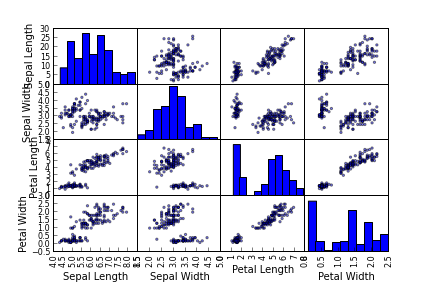
\includegraphics[height=8cm]{stat_cov_corr_01.png}

Iliski oldugu zaman o iliskiye tekabul eden grafikte ``duz cizgiye benzer''
bir goruntu olur, demek ki degiskenlerden biri artinca oteki de artiyor
(eger cizgi soldan sage yukari dogru gidiyorsa), azalinca oteki de azaliyor
demektir (eger cizgi asagi dogru iniyorsa). Eger ilinti yok ise bol
gurultulu, ya da yuvarlak kureye benzer bir sekil cikar. Ustteki grafige
gore yaprak genisligi (petal width) ile yaprak boyu (petal length) arasinda
bir iliski var.

Tanim

$X,Y$ rasgele degiskenlerin arasindaki kovaryans,

$$ Cov(X,Y) = E(X-E(X))(Y-E(Y)) $$

Yani hem $X$ hem $Y$'nin beklentilerinden ne kadar saptiklarini her veri
ikilisi icin, cikartarak tespit ediyoruz, daha sonra bu farklari birbiriyle
carpiyoruz, ve beklentisini aliyoruz (yani tum olasilik uzerinden ne
olacagini hesapliyoruz). 

Ayri ayri $X,Y$ degiskenleri yerine cok boyutlu $X$ kullanirsak, ki
boyutlari $m,n$ olsun yani $m$ veri noktasi ve $n$ boyut (ozellik, oge)
var, tanimi soyle ifade edebiliriz,

$$ \Sigma = Cov(X) = E((X-E(X))^T(X-E(X))) $$



\end{document}
